\section{Results}
\label{sec:results}

\begin{figure*}[ht]
\begin{tabular}{ccc}
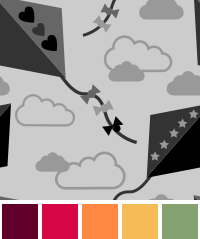
\includegraphics[width=.15\linewidth]{figs/permutationTemplatePalette} & 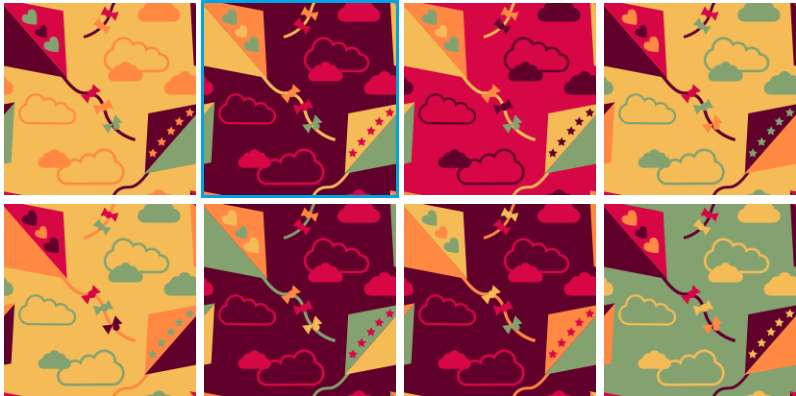
\includegraphics[width=.4\linewidth]{figs/permutationBest8} & 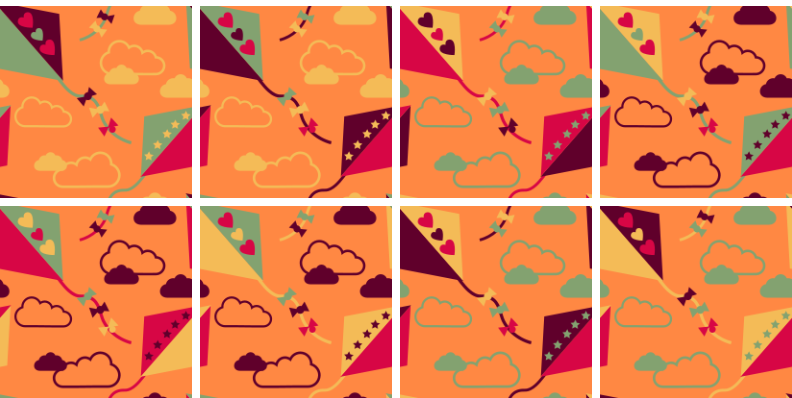
\includegraphics[width=.4\linewidth]{figs/permutationWorst8} %& 
\includegraphics[width=.12\linewidth]{figs/permutationArtist}
  \\
\textbf{(a)} Input Pattern & \textbf{(b)} Highest-scoring assignments & \textbf{(c)} Lowest-scoring assignments %& \textbf{(d)} Artist assignment
\\
\end{tabular}

\caption{Given a segmented image and corresponding palette as input, we use our color model to compute the likelihood of each possible assignment of the palette to the image regions. \textbf{(b)} and \textbf{(c)} show the top-eight and bottom-eight assignments, respectively. The assignment provided by the artist received the second-highest score and is highlighted in blue.}
\label{fig:permutation}
\vspace{-1.0em}
\end{figure*}

\begin{figure}[ht]
\begin{tabular}{cc}

\includegraphics[width=.22\columnwidth]{figs/guidedSearch0Original}&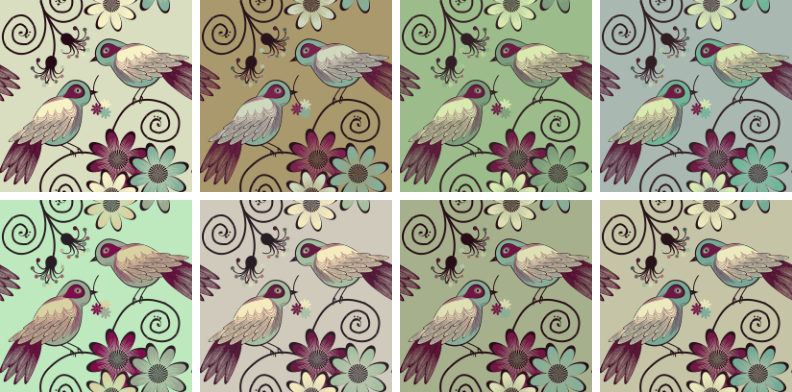
\includegraphics[width=.7\columnwidth]{figs/guidedSearch0MMR}\vspace{0.5em}\\

\includegraphics[width=.22\columnwidth]{figs/guidedSearch1Original}&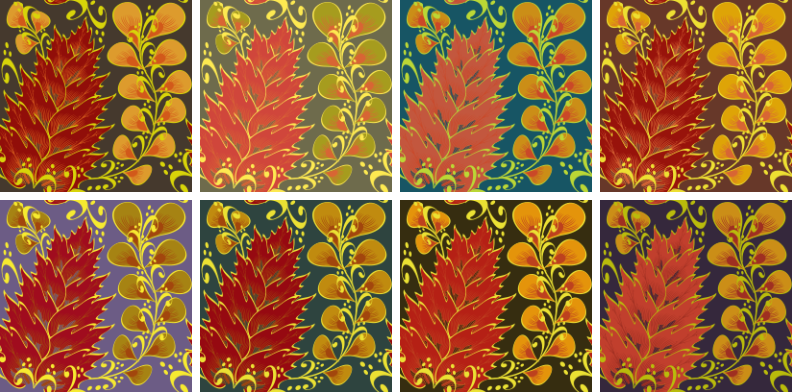
\includegraphics[width=.7\columnwidth]{figs/guidedSearch1MMR}\\
Suggestion&Results\\
\end{tabular}

\caption{An artist provides an initial color assignment and asks for patterns that are similar. We incorporate this request by adding an additional factor to our model, showing eight samples drawn from the new model for each of the suggested images.}
\label{fig:nearbySuggestions}
\vspace{-1.0em}
\end{figure}

\begin{figure}[ht]
\begin{tabular}{ccc} 
Style&Example&Results\\ %\hline
\emph{Bold}&
\includegraphics[width=.145\columnwidth]{figs/styleResultsBoldExample}&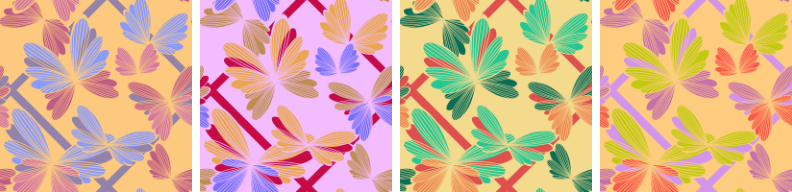
\includegraphics[width=.6\columnwidth]{figs/styleResultsBold}\vspace{0.5em}\\
\emph{Light}&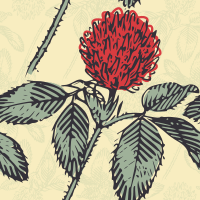
\includegraphics[width=.145\columnwidth]{figs/styleResultsLightExample}&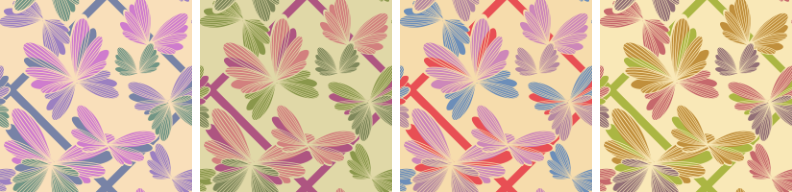
\includegraphics[width=.6\columnwidth]{figs/styleResultsLight}\vspace{0.5em}\\
\emph{Dark}&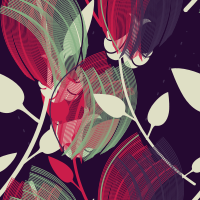
\includegraphics[width=.145\columnwidth]{figs/styleResultsDarkExample}&
\includegraphics[width=.6\columnwidth]{figs/styleResultsDark}\vspace{0.5em}\\
\end{tabular}

\caption{Our model can be trained to match a target color style. In this example, 17 patterns were chosen in three different styles, and a representative image from each style is shown in the second column. A separate model was then trained on each style, and in the third column we show four samples drawn from each model. In each case, our model is able to learn different properties of the desired distribution over colors.}
\label{fig:styleTraining}
\vspace{-1.0em}
\end{figure}

\begin{figure*}[ht]
\begin{tabular}{cc} 
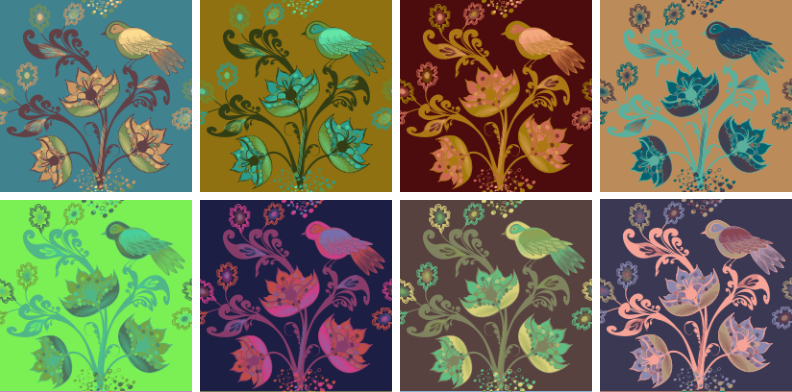
\includegraphics[width=.475\linewidth]{figs/constrainedSearchUnconstrained}&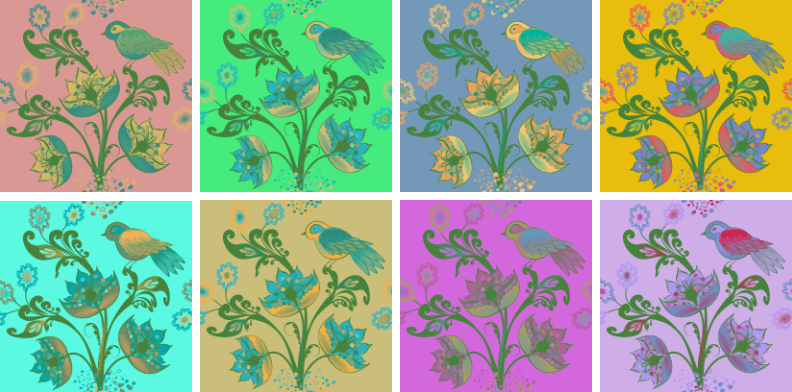
\includegraphics[width=.475\linewidth]{figs/constrainedSearchConstrained}\\
Unconstrained sampling&Constrained sampling\\
\end{tabular}

\caption{An artist coloring a pattern is presented with the results shown on the left, and decides that she does not like results where the stem of the plant is not green. On the right, we use conditional inference to sample from our model subject to the constraint that the desired entry is fixed to a specific color. This is a natural way to incorporate semantic information about regions which cannot be easily learned by our model.}
\label{fig:constrainedInference}
\vspace{-1.0em}
\end{figure*}

Lots of pictures

Quantitative results from reconstruction experiments, etc.

Performance figures? (training time, inference time, etc.)